\documentclass[11pt,a4paper]{article}

\usepackage[margin=0.9in]{geometry}
\usepackage{enumitem}
\usepackage[T1]{fontenc}
\usepackage[utf8]{inputenc}
\usepackage{amsmath,amssymb,amsthm}
\usepackage{booktabs}
\usepackage{graphicx}
\usepackage{subcaption}
\usepackage{listings}
\usepackage{xcolor}
\usepackage[numbers]{natbib}
\usepackage{hyperref}
\usepackage{cleveref}

\graphicspath{{figures/}}

\hypersetup{colorlinks=true,linkcolor=blue!50!black,citecolor=blue!50!black,
            urlcolor=blue!50!black}

\newtheorem{proposition}{Proposition}

% Tighter list and float spacing. This is density, not content: the 10-page
% limit applies to the body, and whitespace is the cheapest thing to give up.
\setlist{topsep=2pt, itemsep=1pt, parsep=0pt}
\setlength{\floatsep}{8pt plus 2pt minus 2pt}
\setlength{\textfloatsep}{10pt plus 2pt minus 2pt}
\setlength{\intextsep}{8pt plus 2pt minus 2pt}
\setlength{\abovecaptionskip}{4pt}
\setlength{\belowcaptionskip}{2pt}

% Shorthands used throughout the report.
\newcommand{\R}{\mathbb{R}}
\newcommand{\muhat}{\hat{\mu}}
\newcommand{\Sig}{\Sigma}
\newcommand{\Ssqrt}{\Sigma^{1/2}}
\newcommand{\one}{\mathbf{1}}
\newcommand{\norm}[1]{\left\lVert #1 \right\rVert}
\newcommand{\prox}{\operatorname{prox}}
\newcommand{\softt}{\mathcal{S}}

% Listing style for the appendix code. `listings`, NOT `minted` -- minted needs
% -shell-escape, which is extra configuration on Overleaf.
\definecolor{codegray}{gray}{0.4}
\definecolor{codegreen}{rgb}{0.0,0.45,0.0}
\definecolor{codeblue}{rgb}{0.0,0.0,0.6}
\lstdefinestyle{pythoncode}{
  language=Python,
  basicstyle=\ttfamily\scriptsize,
  commentstyle=\color{codegreen}\itshape,
  keywordstyle=\color{codeblue}\bfseries,
  stringstyle=\color{codegray},
  numbers=left, numberstyle=\tiny\color{codegray}, numbersep=6pt,
  breaklines=true, breakatwhitespace=false,
  showstringspaces=false,
  frame=single, rulecolor=\color{codegray},
  tabsize=4, captionpos=b,
  upquote=true,
}
\lstset{style=pythoncode}

\begin{document}

% The page counter is reset after the title page (see below), which would make
% hyperref emit two anchors named "page.1". Suppressing anchors on the title
% page avoids that duplicate without affecting any link in the document.
\hypersetup{pageanchor=false}
\begin{titlepage}
\centering
\vspace*{2cm}
{\LARGE\bfseries Sparse and Robust Mean--Variance\\[0.3em]
Portfolio Optimization on the VN100 Universe\par}
\vspace{0.8cm}
{\large A hand-written proximal-subgradient method,\\
cross-verified against an interior-point solver\par}
\vspace{2.5cm}
{\large\bfseries Nguyen To Binh\par}
{\large Student ID: 1010051\par}
\vspace{0.4cm}
{\large Individual project\par}
\vspace{2.5cm}
{\large TODO: Course name and code\par}
\vspace{0.3cm}
{\large TODO: Instructor name\par}
\vfill
{\large \today\par}
\end{titlepage}

% Reset the page counter so that Section 1 begins on page 1. This makes the
% number recorded at \label{sec:endofbody} equal to the main-body page count,
% which is the quantity the 10-page limit applies to.
\setcounter{page}{1}
\hypersetup{pageanchor=true}

\section{Problem Identification}\label{sec:identification}

An investor has one unit of capital and must divide it among the stocks of the VN100 index, the
hundred largest and most actively traded companies listed in Vietnam. Ninety-eight of those
tickers survive the data cleaning of \cref{sec:data}, and the decision is informed by four
years of daily closing prices. What fraction of capital should go into each stock? This is the
general problem of \textbf{portfolio optimization}: choosing capital weights that are, in some
precise sense, the best response to a set of assets' estimated returns and risks.

\textbf{There is no single formula that is best for every market.} The literature offers several
competing answers to what ``best'' should mean --- plain mean--variance efficiency
\citep{markowitz1952}, robustness to estimation error \citep{goldfarb2003}, an explicit penalty
on the number of positions held \citep{tibshirani1996, brodie2009} --- and which of these actually
helps depends on the statistical character of the specific universe being invested in: how noisy
its mean returns are, how correlated its constituents are, how expensive its transaction costs
are. A formula tuned on, say, US large-cap equities carries no guarantee of transferring to a
100-stock Vietnamese universe with a different correlation structure and a different cost profile.
The approach taken here is accordingly not to commit upfront to one fixed formula and assume it is
right, but to state \textbf{one general objective} whose competing terms can each be switched on,
off, or tuned --- collapsing to several named strategies as special cases --- and to let the data
decide, empirically, which configuration of that objective actually performs best on \emph{this}
universe.

The textbook starting point for that general objective is Markowitz mean--variance analysis
\citep{markowitz1952}: estimate each stock's average return and the covariances between stocks,
then trade expected return against portfolio variance. That answer alone is incomplete for three
reasons, and each motivates a term the general formula must be able to switch on:

\textbf{The inputs are estimates, and the mean is a bad one.} An average return computed from a
few years of daily data is noisy. An optimizer handed such an estimate will concentrate capital
in whichever stocks happened to drift upward during the sample, because it cannot distinguish a
genuine tendency from an accident of the period; the resulting portfolio is optimal for the past
and arbitrary for the future. This is the standard explanation for why optimized portfolios so
often fail to beat a naive equal-weight benchmark out of sample \citep{demiguel2009}. A useful
model should therefore be able to ask not only what is best if the estimate is right, but what
remains acceptable if it is wrong.

\textbf{Holding ninety-eight stocks is expensive.} A mathematically optimal portfolio typically
assigns a nonzero weight to every available asset, many of them a fraction of a percent. Each
position must be bought, rebalanced, monitored, and sold, and each transaction costs money. An
investor generally prefers ten or twenty names to ninety-eight even at some cost in theoretical
optimality --- a preference worth encoding as an optional term rather than ignoring or forcing on
unconditionally.

\textbf{Risk still matters.} Variance of the realized portfolio return remains a genuine concern,
and the classical quadratic penalty remains the natural way to express it, in every
configuration.

The goal is therefore twofold: first, to state one model, balancing up to four competing
objectives at once --- expected return, variance, sensitivity to a mis-estimated mean, and the
number of positions held --- general enough that fixing or dropping its terms reproduces several
named strategies rather than requiring a separate formula for each; second, to treat the choice
\emph{among} those configurations as an empirical question specific to VN100 rather than a
theoretical one settled in advance, answered by walk-forward testing several configurations
against each other on this exact universe and reporting which one actually wins here.
\Cref{sec:modeling} states and classifies the general model, \cref{sec:correctness} argues it
represents the problem faithfully and is convex and second-order-cone representable,
\cref{sec:data} describes the data, \cref{sec:insample} solves the model directly with
CVXPY/CLARABEL and reports in-sample results, \cref{sec:backtest} turns the choice of
configuration into that empirical test --- six named variants, walk-forward out of sample, on the
VN100 universe specifically --- and \cref{sec:conclusion} discusses efficiency and limitations.

\section{Problem Modeling}\label{sec:modeling}

\section{Model Correctness}\label{sec:correctness}

\section{Solving the Problem: Method}\label{sec:method}

\subsection{Why a first-order proximal method}

Problem \cref{eq:main} splits as $\min_w f(w) + g(w)$ with
\begin{equation}\label{eq:split}
f(w) = -\muhat^\top w + \kappa\norm{\Ssqrt w}_2 + \gamma\, w^\top \Sig w,
\qquad
g(w) = \lambda\norm{w}_1 + \mathbb{1}\{\one^\top w = 1\},
\end{equation}
where $\mathbb{1}\{\cdot\}$ is $0$ on the feasible set and $+\infty$ off it. The part $f$
admits a subgradient everywhere; $g$ is nonsmooth but, as \cref{prop:jointprox} shows, its
proximal operator can be computed \emph{exactly}. That is precisely the situation proximal
methods are built for \citep{parikh2014}. Folding the budget constraint into $g$ rather than
handling it separately is the decision that makes the method work, for reasons
\cref{sec:proxbug} makes concrete. The solver is pure NumPy: no \texttt{cvxpy},
\texttt{scipy.optimize}, or \texttt{sklearn} routine appears in it, only in the independent
verification of \cref{sec:insample}.

\subsection{The subgradient and step size}

At iterate $w_k$ the method takes a subgradient of $f$:
\begin{equation}\label{eq:subgrad}
v_k \;=\; -\muhat \;+\; 2\gamma\,\Sig w_k
        \;+\; \kappa\,\frac{\Sig w_k}{\norm{\Ssqrt w_k}_2}.
\end{equation}
The third term deserves derivation, being the step at which an implementation is most easily
and most silently wrong. With $u = \Ssqrt w$ and $\Ssqrt$ symmetric, the chain rule gives
\begin{equation}\label{eq:chainrule}
\nabla_w \norm{\Ssqrt w}_2
  \;=\; \bigl(\Ssqrt\bigr)^\top \frac{u}{\norm{u}_2}
  \;=\; \frac{\Ssqrt \Ssqrt w}{\norm{\Ssqrt w}_2}
  \;=\; \frac{\Sig w}{\norm{\Ssqrt w}_2}.
\end{equation}
The numerator is $\Sig w$, the \emph{full} covariance matrix --- not $\Ssqrt w$. Writing
$\Ssqrt w$ is a natural-looking substitution, since $\Ssqrt$ is what appears inside the norm,
and it yields a solver that runs without complaint and converges to the wrong point. Where
$\Ssqrt w = 0$, \cref{eq:chainrule} is undefined; the implementation takes the subgradient to
be $0$, legitimate because the subdifferential of $\norm{\cdot}_2$ at the origin is the closed
unit ball.

The descent step is $z_k = w_k - \alpha_k v_k$ with $\alpha_k = \alpha_0/\sqrt{k+1}$,
$\alpha_0 = 10$. This schedule is square-summable but not summable
($\sum_k\alpha_k = \infty$, $\sum_k\alpha_k^2 < \infty$), the standard sufficient condition for
subgradient-method convergence on a convex objective \citep{boyd2004}. A constant step would
drive the iterates only into a neighbourhood of the optimum whose radius scales with the step,
leaving an objective-gap floor no amount of iteration removes.

\subsection{The joint proximal step}

The remaining piece is the prox of $g$, stated as a proposition because getting it right rather
than approximately right is the technical core of the implementation.

\begin{proposition}[Exact prox of $\ell_1$ plus a budget constraint]\label{prop:jointprox}
Let $z \in \R^N$, let $t > 0$, and let
$\softt_t(x) = \operatorname{sign}(x)\max(|x| - t,\, 0)$ denote coordinate-wise soft
thresholding. The problem
\[
  \prox_{g}(z) \;=\; \arg\min_{w \in \R^N}\;
    \tfrac{1}{2}\norm{w - z}_2^2 + t\norm{w}_1
    \quad \text{subject to} \quad \one^\top w = 1
\]
has the unique solution $w_i = \softt_t(z_i + \nu^\star)$, $i = 1,\dots,N$, where $\nu^\star$
is a root of $h(\nu) := \sum_{i=1}^{N} \softt_t(z_i + \nu) - 1$.
\end{proposition}

The proof is in \cref{app:prox}. It runs in four moves: dualize the single affine constraint;
observe that the Lagrangian then separates across coordinates; solve each one-dimensional
subproblem in closed form, which is where soft thresholding appears; and recover $\nu^\star$ by
a one-dimensional root find, performed by bracketing and \textbf{bisection} to a tolerance of
$10^{-12}$. No closed form for $\nu^\star$ exists, since $h$ is piecewise linear with
data-dependent breakpoints.

Two properties then hold \emph{simultaneously}, which is the whole point of solving the prox
jointly: every coordinate with $|z_i + \nu^\star| \le t$ is set to \textbf{exactly zero} --- a
true floating-point zero, not a small number below a display threshold --- while
$\one^\top w = 1$ holds to the bisection tolerance. Neither is traded against the other.

\subsection{What this replaced: the prox-then-project bug}\label{sec:proxbug}

The first version of the solver did not compute the prox of $g$ jointly. It handled the two
nonsmooth pieces in sequence: soft-threshold first, then restore feasibility by a separate
Euclidean projection onto $\{\one^\top w = 1\}$, adding the uniform offset
$(1 - \one^\top w_{\text{half}})/N$ to \emph{every} coordinate. The failure is immediate once
stated: that offset is added to the coordinates soft thresholding had just set to zero,
reviving them. The returned portfolio satisfies the budget constraint and looks plausible, but
it is not sparse and it is not the minimizer.

The effect was not marginal. Against the independent solver of \cref{sec:insample}, on real
data with identical parameters, the two-step version reported \textbf{48 active positions where
the reference solver reported 9}, with an objective gap of \textbf{2.7--6\%}.

The general statement is that $\prox_{f_1 + f_2} \neq \prox_{f_1} \circ \prox_{f_2}$: the
proximal operator of a \emph{sum} of nonsmooth functions is not the composition of the
individual operators, and the two do not commute. When an objective carries several nonsmooth
components at once --- here an $\ell_1$ penalty and an affine constraint --- the prox of the sum
must be solved as one problem, which is what \cref{prop:jointprox} does.

Two points are worth drawing out. Each individual step in the broken version was correct in
isolation: soft thresholding is the right prox for $\ell_1$, and the uniform offset is the right
projection onto the hyperplane. Only their composition was wrong, which is why the error
survived inspection. And the output gave no signal --- a portfolio of 48 positions summing to
one is not visibly defective. The bug was found only by comparison against an independently
implemented solver, which is the argument for \cref{sec:insample} existing at all.

\subsection{Best-iterate tracking and the long-only variant}

A subgradient method is not a descent method: $f(w_{k+1}) \le f(w_k)$ is not guaranteed, and
the objective oscillates, particularly while $\alpha_k$ is large. The implementation therefore
records $\min_{j \le k} f(w_j)$ with the iterate attaining it and returns that, not the last
iterate, which would report an objective worse than the method achieved. Termination is judged
on the same quantity: the loop stops once the relative change in $\min_{j\le k} f(w_j)$ stays
below $10^{-8}$ for $100$ consecutive iterations.

For the backtest of \cref{sec:backtest}, $w \ge 0$ is added and the feasible set becomes the
probability simplex. Two things change. The proximal step becomes Euclidean projection onto
that simplex, computed by the standard sort-and-threshold algorithm \citep{duchi2008}. And the
$\ell_1$ term disappears: on the simplex $\norm{w}_1 = \one^\top w = 1$ identically, so
$\lambda\norm{w}_1$ contributes the constant $\lambda$ regardless of which feasible $w$ is
chosen and cannot influence the argmin. Hence $\lambda$ is dropped from the hyperparameter grid
in \cref{sec:backtest}: searching over it would consume compute and change nothing. The
subgradient \cref{eq:subgrad} is reused unchanged. The complete algorithm is stated as
pseudocode in \cref{alg:proxsub}.

\section{Data}\label{sec:data}

Constituents of the VN100 index were obtained through the \texttt{vnstock} library
\citep{vnstock}. Of the \textbf{100} listed constituents, $N = 98$ tickers survive cleaning ---
two are dropped for insufficient trading history within the 4-year window. The price panel
spans \textbf{2022-07-26 to 2026-07-24} ($997 \times 98$), and the derived simple-return panel
spans \textbf{2022-07-27 to 2026-07-24} ($965 \times 98$). All results in this report use that
return panel.

One structural limitation should be stated before any result. The \emph{current} VN100
is applied backward across the full four years, so companies that left the index or
were delisted during the period are absent. The sample is biased toward survivors, which tends
to flatter any strategy evaluated on it --- including the benchmark. This is revisited in
\cref{sec:conclusion}.

\section{In-Sample Results and Cross-Verification}\label{sec:insample}

\subsection{Estimating the inputs}

$\muhat$ is the column-wise sample mean of the return panel and $\Sig$ its sample covariance
($\text{ddof} = 1$), symmetrized. The square root $\Ssqrt$ is built by \textbf{eigendecomposition
rather than Cholesky factorization}: a sample covariance estimated with $N = 98$ from $T = 965$
observations is positive \emph{semi}definite at best and in floating point carries a few
marginally negative eigenvalues, on which Cholesky --- requiring strict positive definiteness ---
simply fails. The implementation computes $\Sig = V\operatorname{diag}(\ell)V^\top$, clips
negative $\ell_i$ to zero, and sets $\Ssqrt = V\operatorname{diag}(\sqrt{\ell})V^\top$,
reconstructing $\Sig$ to $\norm{\Ssqrt\Ssqrt - \Sig}_F / \norm{\Sig}_F = 1.831 \times 10^{-15}$.

\subsection{Solver behaviour and the effect of $\lambda$}

\Cref{tab:demo} reports two representative solves. In both, $\one^\top w = 1$ holds to
$10^{-12}$ and the reported zeros are \textbf{exact} zeros produced by the proximal step, not
small values below a display threshold. That is the practical payoff of \cref{prop:jointprox}:
the sparsity is real, so the count of nonzero weights is a count of positions the investor would
actually open.

\begin{table}[htbp]
\centering
\caption{Two representative solves on the full return panel.}
\label{tab:demo}
\small
\begin{tabular}{@{}lrrrr@{}}
\toprule
$(\kappa,\gamma,\lambda)$ & Iterations & Objective & Active $(|w_i| > 10^{-4})$ & Exact zeros \\
\midrule
$(1,\, 5,\, 0.01)$ & 528  & 0.015302 & 17 / 98 & 81 / 98 \\
$(0,\, 5,\, 0.10)$ & 2113 & 0.099071 & 10 / 98 & 88 / 98 \\
\bottomrule
\end{tabular}
\end{table}

\begin{figure}[htbp]
\centering
\begin{subfigure}[t]{0.44\textwidth}
  \centering
  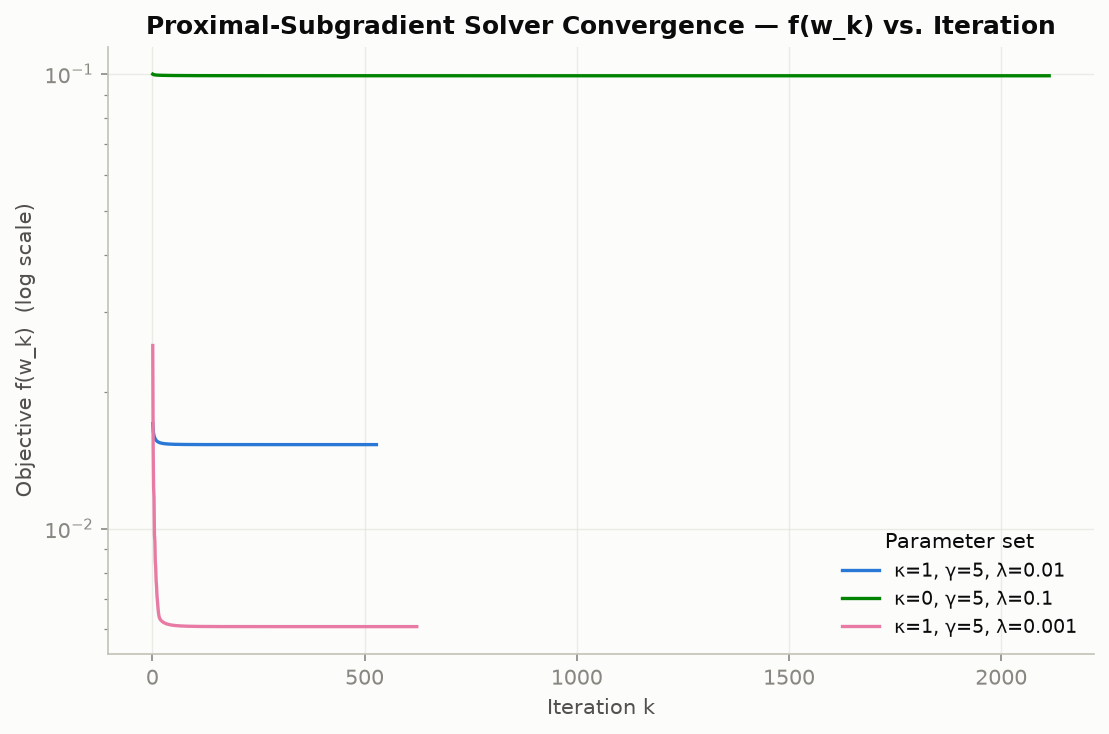
\includegraphics[width=\textwidth]{fig2_convergence.png}
  \caption{Objective against iteration count.}
  \label{fig:convergence}
\end{subfigure}
\hfill
\begin{subfigure}[t]{0.44\textwidth}
  \centering
  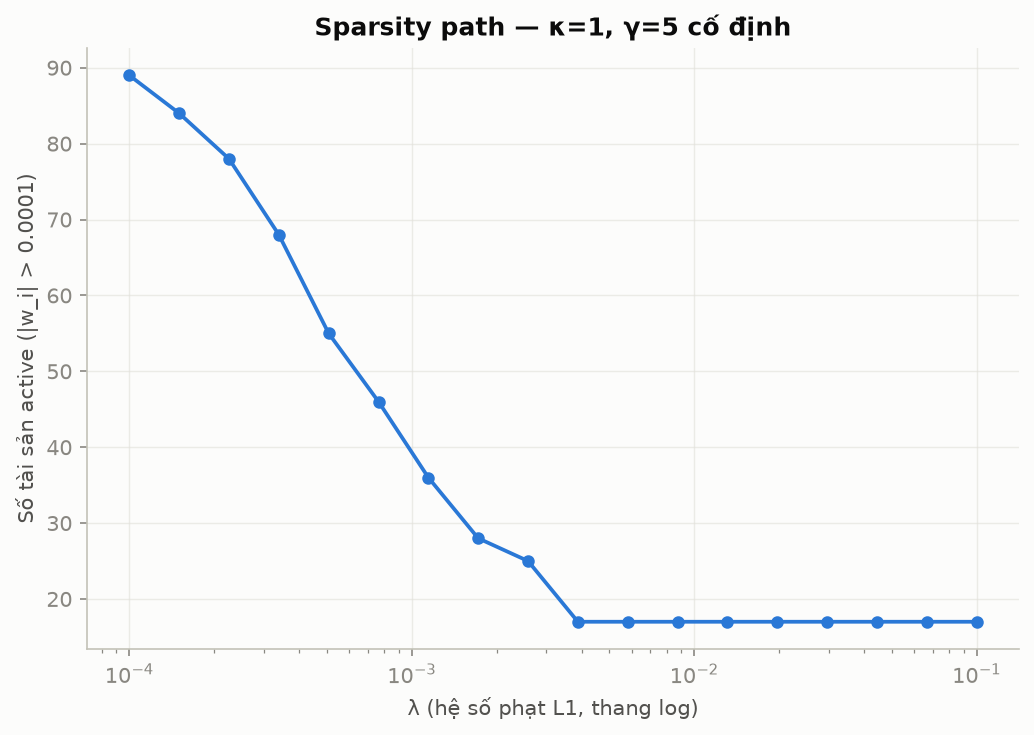
\includegraphics[width=\textwidth]{fig3_sparsity_path.png}
  \caption{Active positions against $\lambda$.}
  \label{fig:sparsity}
\end{subfigure}
\caption{Left: convergence; the non-monotone early phase is expected of a subgradient method and
is why the solver returns the best iterate. Right: the sparsity path.}
\label{fig:solver}
\end{figure}

\Cref{fig:sparsity} traces active positions as $\lambda$ sweeps a logarithmic grid. The count
falls as $\lambda$ rises but \textbf{not strictly monotonically}, for a structural rather than
numerical reason: $\lambda$ enters only through the threshold $t = \alpha_k\lambda$, and raising
$t$ also shifts the multiplier $\nu^\star$ enforcing the budget constraint in
\cref{prop:jointprox}, so a larger $\lambda$ can move $z_i + \nu^\star$ far enough for a
coordinate to re-enter the active set even as others leave. The trend is unambiguous; the
monotonicity is not, and the figure is reported as it is rather than smoothed.

\subsection{The effect of the robust term}

Raising $\kappa$ from $0$ to $1$ with $\gamma, \lambda$ fixed \textbf{increases} both the number
of active positions and the Herfindahl--Hirschman concentration index: the portfolio becomes
\emph{more} concentrated, where the folk intuition --- robust means cautious means diversified
--- predicts the opposite. The mechanism is the degree-one homogeneity of
\cref{eq:robust-derivation}: because $\kappa\norm{\Ssqrt w}_2$ is a norm rather than a squared
norm, its subgradient $\kappa\,\Sig w / \norm{\Ssqrt w}_2$ does \emph{not} shrink in magnitude as
$\norm{w}$ shrinks, unlike the variance gradient $2\gamma\Sig w$, so it exerts a scale-independent
pull in a fixed direction --- which, given a covariance matrix dominated by a single market
factor, is served more efficiently by concentrating weight along a low-variance combination of a
few names than by spreading it across many correlated ones. This is an empirical observation on
one dataset with a plausible mechanism, \emph{not} a theorem about every $\Sig$.
\Cref{app:robust} gives the figure.

\subsection{Cross-verification against an interior-point solver}

The method of \cref{sec:method} is first-order, hand-written, and specific to this problem.
CLARABEL \citep{clarabel2024}, invoked through CVXPY \citep{diamond2016}, is a general-purpose
second-order interior-point solver operating on the conic reformulation \cref{eq:socp}. They
share no code, no algorithmic family, and no failure modes, and \cref{sec:correctness}
established that the optimal value is unique --- so two correct solvers must agree on it.
Agreement on the objective is the weaker test; agreement on the \textbf{active set} is far
stronger, because the support is a discrete object that a numerically close but structurally
wrong solution --- such as one from the scheme of \cref{sec:proxbug} --- will generally get wrong
even while landing near the right objective value. That is exactly how the bug was caught.

\begin{table}[htbp]
\centering
\caption{Hand-written solver against CVXPY/CLARABEL. Jaccard $= 1.00$ means the supports are
identical. The full table, with $\ell_\infty$ weight distances and iteration counts, is in
\cref{app:verification}.}
\label{tab:cvxpy}
\small
\begin{tabular}{@{}rrrrrrrr@{}}
\toprule
$\kappa$ & $\gamma$ & $\lambda$ & $f_{\text{hand}}$ & Rel.\ gap
  & Active (hand) & Active (CVXPY) & Jaccard \\
\midrule
1   & 5  & 0.01  & 0.0153016 & $1.92 \times 10^{-7}$  & 17 & 17 & 1.00 \\
0   & 5  & 0.10  & 0.0990708 & $7.75 \times 10^{-6}$  & 10 & 10 & 1.00 \\
1   & 5  & 0.001 & 0.0060877 & $2.44 \times 10^{-7}$  & 39 & 39 & 1.00 \\
2   & 10 & 0.05  & 0.0607131 & $-1.66 \times 10^{-8}$ & 16 & 16 & 1.00 \\
0.5 & 1  & 0.02  & 0.0225015 & $1.82 \times 10^{-6}$  & 18 & 18 & 1.00 \\
1   & 5  & 0     & 0.0045395 & $5.14 \times 10^{-7}$  & 98 & 98 & 1.00 \\
\bottomrule
\end{tabular}
\end{table}

The result is unambiguous: the \textbf{maximum relative objective gap is $0.000775\%$} and the
\textbf{active sets match exactly on all six of six parameter sets}, every run reporting
convergence; \cref{fig:proxcvx} in \cref{app:verification} shows the individual weights lying on
the line $y = x$.

The last row is a deliberate control: with $\lambda = 0$ the $\ell_1$ penalty is off and both
solvers return a fully dense portfolio of 98 active positions. Without it, identical supports
could in principle reflect nothing more than two methods trivially zeroing the same coordinates;
the dense case shows the agreement survives when there is no sparsity to agree about.

One detail deserves disclosure. CVXPY rejects a covariance matrix that is not strictly positive
semidefinite in floating point, so the code wraps $\Sig$ in \texttt{cp.psd\_wrap} to suppress
that check. This relaxes a numerical tolerance --- the same concession as clipping eigenvalues
when forming $\Ssqrt$ --- and does not alter the data passed to either solver.

\section{Walk-Forward Out-of-Sample Backtest}\label{sec:backtest}

\section{Discussion, Limitations, and Conclusion}\label{sec:conclusion}

\subsection{Computational efficiency}

Across the verification grid the hand-written solver required between \textbf{222 and 2113}
iterations. Per-iteration cost is dominated by a single matrix--vector product $\Sig w$ at
$O(N^2)$, plus the bisection of \cref{prop:jointprox} at $O(N \log(1/\epsilon))$; no matrix
factorization occurs anywhere inside the loop, and memory traffic is one $N \times N$ read per
iteration.

The contrast with the interior-point method is the expected one in kind: CLARABEL converges in
a few dozen iterations rather than hundreds, but each iteration forms and factorizes a KKT
system at roughly $O(N^3)$. It would be convenient to conclude that the first-order method
therefore wins, and the data does not support that. At $N = 98$ a dense $98 \times 98$
factorization is trivial for a modern machine, the interior-point solver is entirely practical,
and neither method is anywhere near a wall-clock bottleneck. The first-order method's advantage
here is that it is transparent and was built from the problem structure rather than invoked;
its asymptotic advantage would become a real one only at $N$ in the thousands, where
factorization cost dominates and the $O(N^2)$ per-iteration profile starts to matter.

\subsection{Solution quality}

The solver produces exact zeros rather than thresholded small values, satisfies the budget
constraint to $10^{-12}$, matches an independently implemented interior-point solver to a
maximum relative objective gap of $7.75 \times 10^{-6}$, and reproduces its active set exactly
on every parameter set tested (\cref{tab:cvxpy}). For a convex problem with a unique optimal
value, that combination is strong evidence of correctness.

\subsection{Limitations}

\begin{itemize}
  \item \textbf{Survivorship bias.} The current VN100 membership is applied backward over four
        years, so delisted and removed tickers are absent from the universe.
  \item \textbf{$\muhat$ remains a poor estimator.} The sample mean has high variance over a
        short window. The robust term blunts the consequences of this; it does not remove them,
        and no term in \cref{eq:main} can.
  \item \textbf{The $\kappa$ finding is empirical.} The increase in concentration reported in
        \cref{sec:insample} is an observation on one covariance structure with a plausible
        mechanism, not a general result.
  \item \textbf{The out-of-sample window is short.} Roughly 24 months spanning a single market
        regime. The conclusions of \cref{sec:backtest} cannot be extrapolated to other cycles.
  \item \textbf{Validation overfitting.} Selecting $(\kappa,\gamma)$ on a six-month window is a
        mild form of fitting to the validation set, inherent to short-window walk-forward
        rather than a defect of this implementation --- and, as \cref{sec:backtest} shows, it
        is the direct cause of the turnover that drives the cost disadvantage.
  \item \textbf{A single historical path.} No block bootstrap or resampling was performed, so
        no confidence interval accompanies the reported Sharpe ratio or drawdown.
  \item \textbf{Costs are modelled crudely.} A flat $0.20\%$ of turnover, with no market-impact
        or slippage term and no dependence on order size or liquidity.
\end{itemize}

\subsection{Conclusion}

The portfolio selection problem was formulated as a convex, second-order-cone representable
program in which the robust term is derived as an exact worst-case objective over an
ellipsoidal uncertainty set rather than assumed, and in which the $\ell_1$ penalty serves
simultaneously as a convex surrogate for the number of holdings and as a cap on gross leverage.
A proximal-subgradient method was implemented in pure NumPy, resting on an exact joint
proximal operator for the $\ell_1$ penalty and the budget constraint taken together
(\cref{prop:jointprox}). That solver reproduces an independent interior-point solver's optimal
value to $7.75 \times 10^{-6}$ relative gap and its active set exactly, on every parameter set
tested. Out of sample, the resulting long-only strategy beat an equal-weight benchmark on a
risk-adjusted basis over 494 trading days --- by a real but modest margin, at materially higher
volatility, deeper drawdown, and roughly seven times the transaction cost.

The methodological lesson is the one from \cref{sec:proxbug}. The original solver composed two
individually correct operations --- soft thresholding and projection onto the budget hyperplane
--- into an incorrect one, and returned portfolios that were feasible, plausible, and wrong by
several percent in objective and by a factor of five in the number of positions held. Nothing
in the output revealed it. It was found only by solving the same problem a second time with an
unrelated algorithm and comparing. For convex problems, where a unique optimum makes such a
comparison decisive, building that independent check is worth more than any amount of
inspection of the primary implementation.

\label{sec:endofbody}


\bibliographystyle{plainnat}
\bibliography{refs}

\appendix
\section{Data Cleaning Detail}\label{app:data}

\Cref{fig:dataoverview} summarizes the cleaned return panel: the distribution of daily returns
pooled across tickers, the cross-sectional correlation structure, the number of tickers
reporting on each session, and the per-ticker volatility spread. The dominant single factor
visible in the correlation panel --- most pairs of VN100 constituents are strongly positively
correlated --- is the structural feature invoked in \cref{sec:insample} to explain why the
robust term concentrates rather than diversifies on this universe.

\begin{figure}[htbp]
\centering
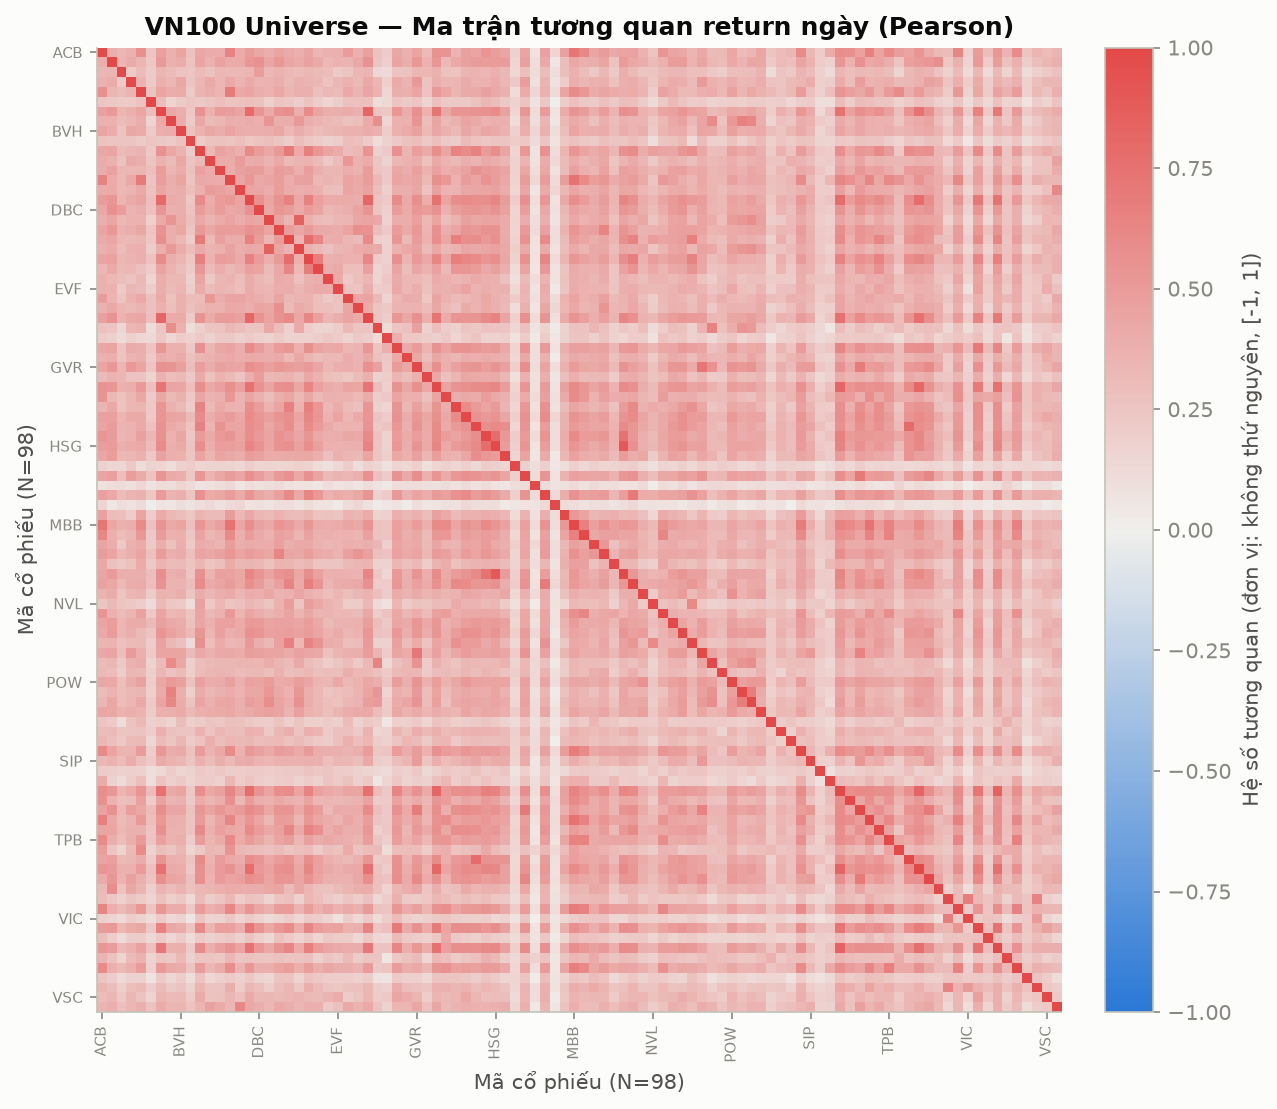
\includegraphics[width=\textwidth]{fig1_data_overview.png}
\caption{Overview of the cleaned VN100 return panel: 98 tickers, 965 sessions,
2022-07-27 to 2026-07-24.}
\label{fig:dataoverview}
\end{figure}

\paragraph{Zero-return diagnostic.}
Beyond the two vendor defects described in \cref{sec:data}, the per-ticker proportion of
exactly-zero return sessions was ranked across all 98 tickers. The purpose was diagnostic: a
single ticker dominating the zero counts would indicate a per-ticker feed problem --- a stock
suspended from trading, or a symbol whose price series is stale --- which is a different defect
requiring a different remedy from the market-wide repeated-price artifact that the $90\%$
filter targets. No such dominance was found; zero returns are distributed across tickers at
levels consistent with ordinary low-liquidity sessions and price-limit days on an exchange with
daily price bands.

\paragraph{Why the holiday filter is statistical.}
A \texttt{dayofweek >= 5} test removes weekends but cannot remove Vietnamese public holidays
that fall on a weekday. Hard-coding a holiday calendar would require annual maintenance and
would fail silently once out of date. The implemented rule --- drop any session on which at
least $90\%$ of tickers post exactly zero return --- keys on the observable signature of the
defect rather than on the calendar. The threshold is deliberately high: genuine market-wide
flat days are possible in principle, and a lower threshold risks discarding real sessions. As
noted in \cref{sec:data}, this filter removes no rows from the present panel.

\section{Additional In-Sample Figures}\label{app:robust}

\begin{figure}[htbp]
\centering
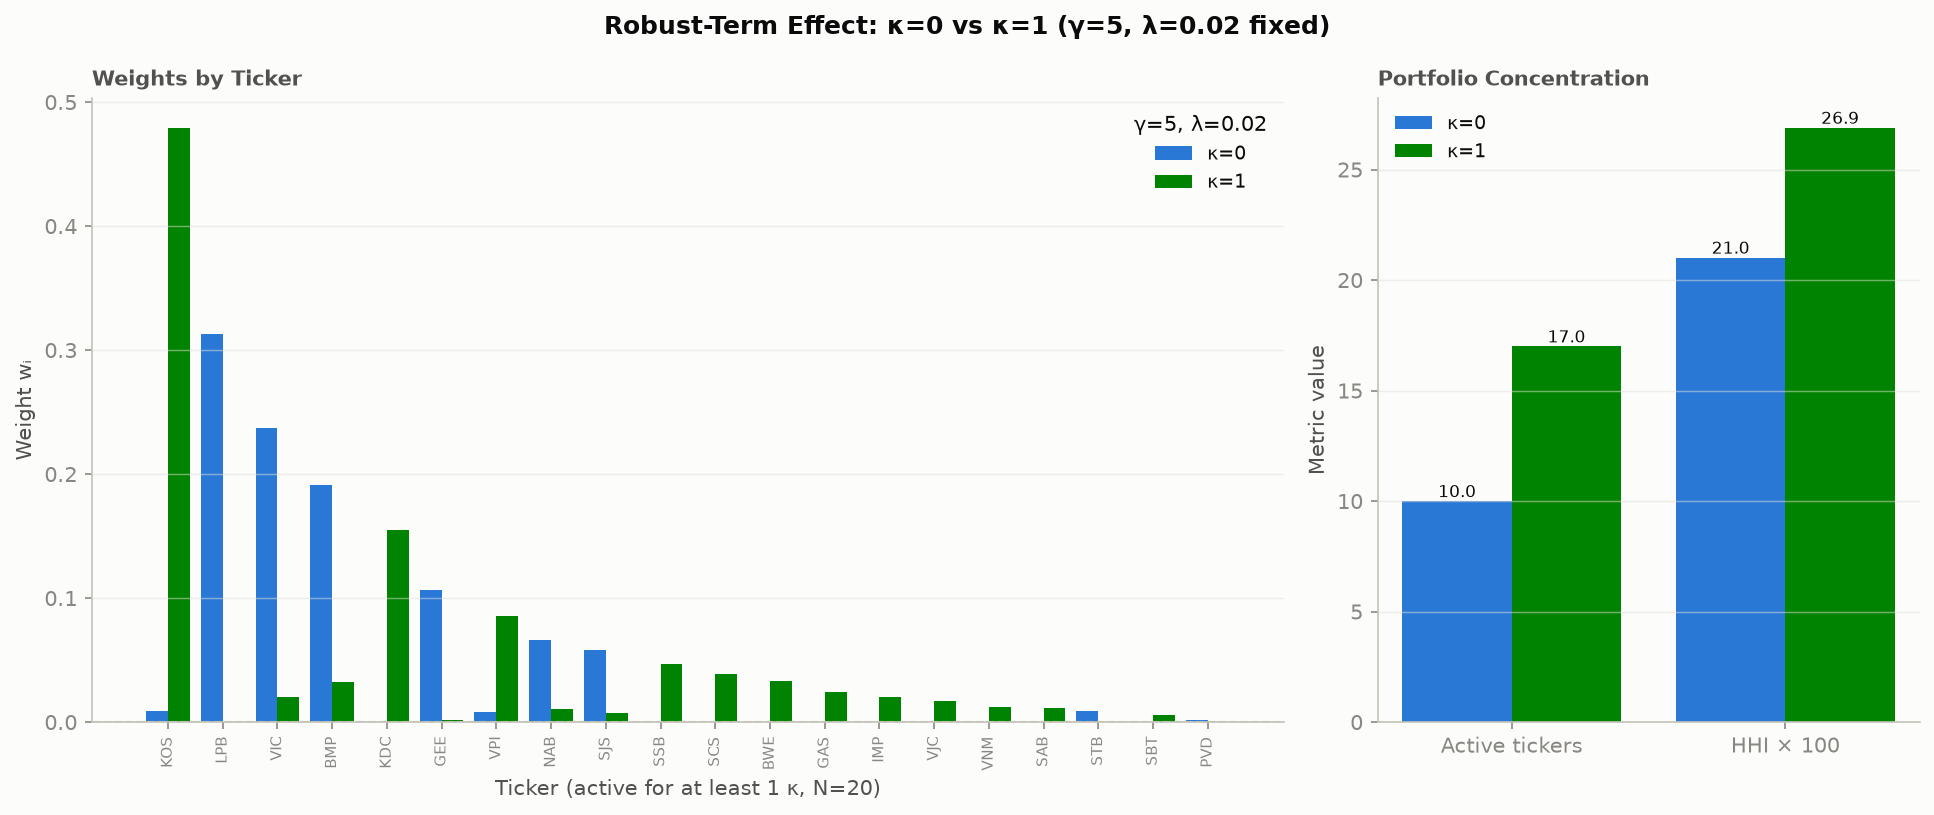
\includegraphics[width=0.6\textwidth]{fig5_robust_effect.png}
\caption{Active positions and Herfindahl--Hirschman index as $\kappa$ increases from $0$ to $1$
with $\gamma$ and $\lambda$ held fixed. Both rise: the portfolio becomes more concentrated, not
more diversified. The mechanism --- degree-one homogeneity of the robust term --- is discussed in
\cref{sec:insample}.}
\label{fig:robust}
\end{figure}

\begin{figure}[htbp]
\centering
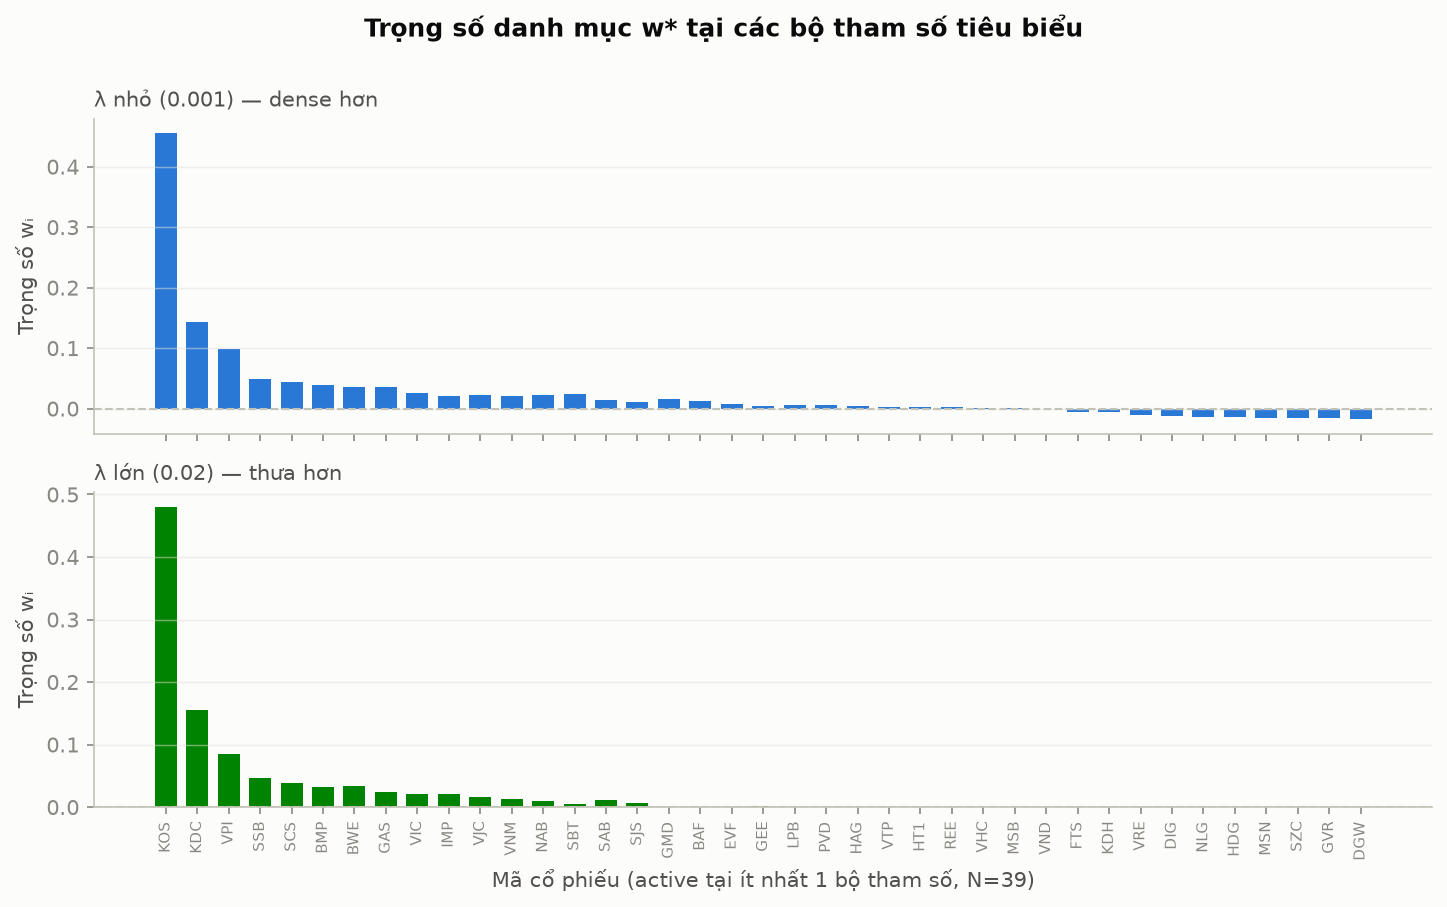
\includegraphics[width=0.75\textwidth]{fig4_weights_bar.png}
\caption{Portfolio weights at a small $\lambda$ (denser) against a large $\lambda$ (sparser). The
large-$\lambda$ portfolio concentrates in the few tickers with the best marginal contribution to
the objective; the remaining weights are below the $10^{-4}$ active threshold, not merely small
relative to the active ones.}
\label{app:weights}
\end{figure}

\section{Explicit Objectives for Each Backtest Variant}\label{app:variants}

\Cref{tab:variants} summarizes the six variants of \cref{sec:backtest}; this appendix gives each
one's objective explicitly, each obtained from \cref{eq:main} by fixing or dropping specific
terms --- no variant introduces a term not already present in the general model. A and B
additionally impose $w\ge0$ here, and pick up the concentration constraint of \cref{sec:cap} only
in \cref{tab:beforeafter}. C and D solve no optimization problem at all.

\textbf{A} (robust, long-only) --- $\kappa$ and $\gamma$ searched, $\lambda\equiv0$ (vacuous under
the simplex, \cref{eq:leverage}):
\[
\min_{w\ge0,\ \mathbf1^\top w=1}\ -\muhat^\top w
  \;+\; \underbrace{\kappa\norm{\Ssqrt w}_2}_{\text{robustness}}
  \;+\; \underbrace{\gamma\, w^\top\Sig w}_{\text{variance}}
\]

\textbf{B} (classical, long-only) --- $\kappa\equiv0$ (robust term off), $\gamma$ searched,
$\lambda\equiv0$ (same vacuity as A: B is exactly A with the robust term switched off, nothing
else differs):
\[
\min_{w\ge0,\ \mathbf1^\top w=1}\ -\muhat^\top w
  \;+\; \underbrace{\gamma\, w^\top\Sig w}_{\text{variance}}
\]

\textbf{C} (equal-weight $1/N$) and \textbf{D} (VN100 buy\&hold) --- $w_i = 1/N$ for every $i$, no
objective solved: C resets to $1/N$ every month, D sets it once and lets it drift untouched.

\textbf{E} (sparse-only, long-short) --- $\kappa\equiv0$ (robust off), $\gamma$ searched, $\lambda$
searched over a real grid, the only variant where sparsity is a \emph{designed} choice rather than
a byproduct:
\[
\min_{\mathbf1^\top w=1}\ -\muhat^\top w
  \;+\; \underbrace{\gamma\, w^\top\Sig w}_{\text{variance}}
  \;+\; \underbrace{\lambda\norm{w}_1}_{\text{sparsity / leverage}}
\]

\textbf{F} (full equation, long-short) --- $\kappa$, $\gamma$, $\lambda$ all searched:
\cref{eq:main} exactly as stated, no term fixed and no exposure constraint added, which
\cref{sec:ef} shows is precisely the combination that fails:
\[
\min_{\mathbf1^\top w=1}\ -\muhat^\top w
  \;+\; \underbrace{\kappa\norm{\Ssqrt w}_2}_{\text{robustness}}
  \;+\; \underbrace{\gamma\, w^\top\Sig w}_{\text{variance}}
  \;+\; \underbrace{\lambda\norm{w}_1}_{\text{sparsity / leverage}}
\]

\section{Transaction-Cost Worked Example}\label{app:timeline}

The rolling-window mechanism itself, with the month-numbering table, is given where it is first
used, in \cref{sec:backtest}'s Design subsection (\cref{tab:timeline}). This appendix works
through the turnover and transaction-cost calculation in detail.

At each rebalance, \texttt{src/backtest.py} computes turnover and cost from the full weight
vector as
\begin{lstlisting}[language=Python, numbers=none]
turnover = float(np.abs(w_start - prev).sum())   # sum of |delta w_i| over ALL 98 tickers
cost     = fee * turnover                        # one multiplication
\end{lstlisting}
where \texttt{w\_start} is the new target weight vector for this period and \texttt{prev} is
the \emph{drifted} portfolio at the close of the previous period --- the weights actually held
just before rebalancing, after a month of price movement, not the previous period's target.
This distinction matters: a portfolio that started last month exactly at its target can drift
several points away from it through price movement alone, and correcting that drift is real
turnover the investor must pay for.

\textbf{Example.} Suppose two of the 98 tickers have drifted to $60\%$ and $40\%$ of portfolio
value by the close of the previous period, and the new target for this period is $30\%$ and
$70\%$ (every other ticker unchanged, contributing $0$ to the sum):
\begin{equation}
\text{turnover} = |30\%-60\%| + |70\%-40\%| = 30\% + 30\% = 60\%,
\qquad
\text{cost} = 0.20\% \times 60\% = 0.12\%
\end{equation}
of portfolio value, deducted from the return of the \emph{first trading day} of the new holding
period only --- the portfolio then drifts untouched, with no further trading, for the rest of
the month. For the very first period of the backtest there is no previous portfolio to compare
against, so \texttt{prev} is treated as all zero and turnover $= \sum_i w_i = 1$ exactly (a full
purchase from cash), matching the $100\%$ first-period turnover stated in \cref{sec:backtest}.

\section{Why Transaction Cost Is Kept External to the Objective}\label{app:turnover-design}

\Cref{sec:interpretation} treats transaction cost as a friction applied \emph{after} $w^\star$ is
chosen --- \cref{eq:main} has no term that sees $w_{\text{prev}}$ at all, so the optimizer that
picks $\gamma=1$ this month has no way to know that doing so will force a $60\%$ turnover against
last month's holdings. The natural alternative is to add a turnover penalty
$\eta\norm{w-w_{\text{prev}}}_1$ directly to \cref{eq:main} at each rebalance, letting the
optimizer trade expected return against \emph{both} risk and rebalancing cost simultaneously,
the standard treatment in the transaction-cost portfolio literature. Three reasons this report
keeps cost external instead:

First, \cref{eq:main} is stated and solved once in \cref{sec:insample} as a single-period
problem, and $w_{\text{prev}}$ is meaningful only in the multi-period walk-forward setting of
\cref{sec:backtest} --- folding it in would mean the core model of \cref{sec:modeling} is no
longer the same model actually deployed, which this report's structure deliberately avoids.
Second, $\eta$ would be a fourth hyperparameter selected on the same six-month validation window
already shown (\cref{sec:results7}, \cref{fig:selectedparams}) to select $\gamma$ unstably ---
adding a cost-aware term without first fixing that instability risks fitting $\eta$ to six months
of noise rather than to a genuine cost--return trade-off. Third, and most concretely, the
concentration cap of \cref{sec:cap} was added \emph{because} of a diversification concern
(\cref{app:backtest}), not a cost concern, yet it happens to cut A's and B's turnover as a side
effect --- keeping cost external keeps that attribution clean: \cref{tab:beforeafter}'s
improvement is demonstrably from the cap, not confounded with a simultaneously-tuned cost
penalty. A cost-aware variant, $\eta\norm{w-w_{\text{prev}}}_1$ added once the $\gamma$-selection
instability above is addressed, is left as the natural next extension rather than folded in here.

\section{Backtest Diagnostics}\label{app:backtest}

\begin{table}[htbp]
\centering
\caption{Method B (uncapped), active positions by month --- the trace behind the concentration
constraint of \cref{sec:cap}. Mean $7.56$, range $1$--$14$.}
\label{tab:bmonthly}
\small
\begin{tabular}{@{}lr@{\hspace{18pt}}lr@{\hspace{18pt}}lr@{}}
\toprule
Month & $n$ & Month & $n$ & Month & $n$ \\
\midrule
2024-07 & 12 & 2025-02 & 1  & 2025-09 & 14 \\
2024-08 & 10 & 2025-03 & 2  & 2025-10 & 2  \\
2024-09 & 9  & 2025-04 & 2  & 2025-11 & 9  \\
2024-10 & 9  & 2025-05 & 3  & 2025-12 & 3  \\
2024-11 & 7  & 2025-06 & 12 & 2026-01 & 10 \\
2024-12 & 12 & 2025-07 & 10 & 2026-02 & 11 \\
2025-01 & 12 & 2025-08 & 12 & 2026-03 & 4  \\
        &    &         &    & 2026-04 & 2  \\
        &    &         &    & 2026-05 & 7  \\
        &    &         &    & 2026-06 & 6  \\
        &    &         &    & 2026-07 & 8  \\
\bottomrule
\end{tabular}
\end{table}

\begin{figure}[htbp]
\centering
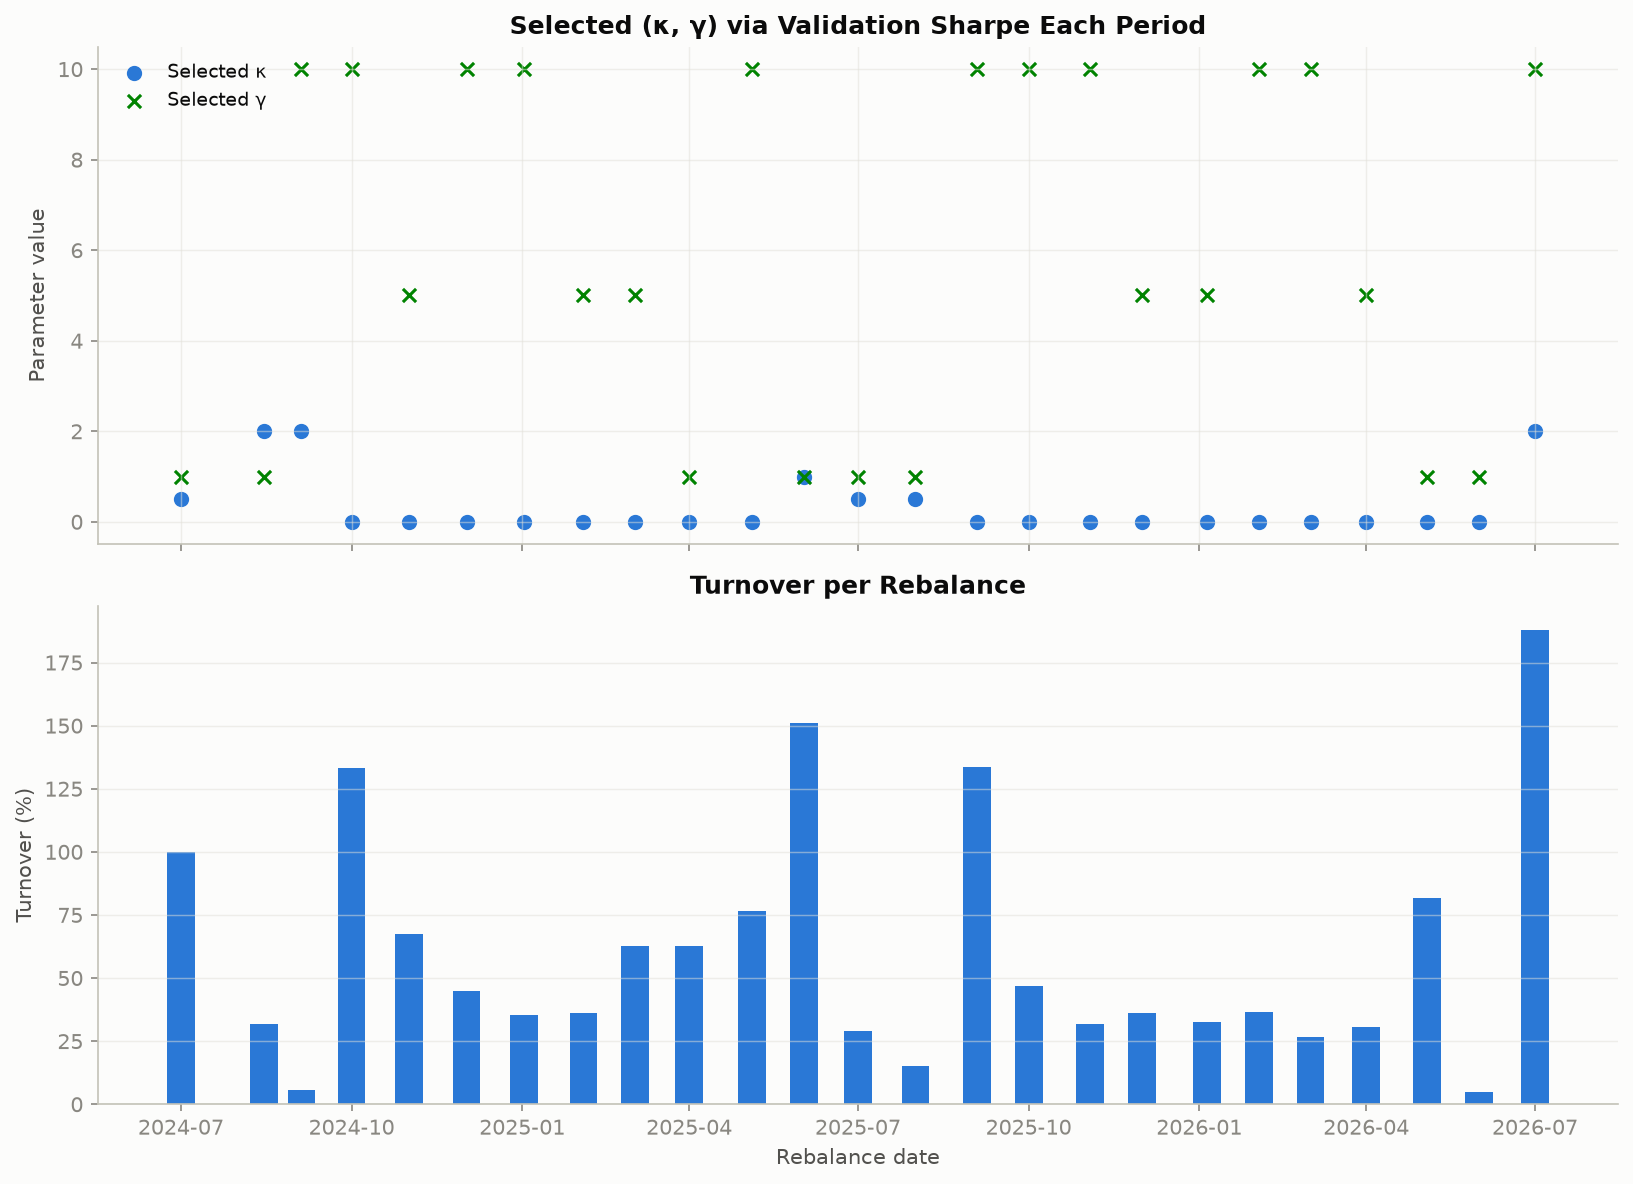
\includegraphics[width=0.82\textwidth]{fig9_selected_params.png}
\caption{Method A: $(\kappa,\gamma)$ selected by validation Sharpe at each monthly rebalance, and
the resulting turnover. $\gamma$ moves across $\{1, 5, 10\}$ between adjacent periods without
settling, and each move rewrites a meaningful share of the portfolio even under the concentration
cap of \cref{sec:backtest} --- the visual evidence for the turnover diagnosis in
\cref{sec:results7}. $\kappa = 0$ is selected in 18 of 25 periods, consistent with the finding
that the robust term does not earn its keep on this data.}
\label{fig:selectedparams}
\end{figure}

\section{Code Listings}\label{app:code}

The three modules below implement the core contribution of this report: the estimators feeding
\cref{eq:main}, the proximal-subgradient solver of \cref{sec:algorithm}, and the walk-forward
backtest of \cref{sec:backtest}. Full source, with tests, is in the accompanying code submission;
these are reproduced verbatim.

\subsection{\texttt{src/estimators.py}}
\lstinputlisting[language=Python]{code/estimators.py}

\subsection{\texttt{src/prox\_solver.py}}
\lstinputlisting[language=Python]{code/prox_solver.py}

\subsection{\texttt{src/backtest.py}}
\lstinputlisting[language=Python]{code/backtest.py}

\section{Reproduction}\label{app:repro}

\begin{lstlisting}[language={}, basicstyle=\ttfamily\small, numbers=none, frame=single]
python3 -m venv .venv && source .venv/bin/activate
pip install -r requirements.txt
python -m src.data_loader     # only if data/*.parquet is absent
pytest tests/ -v              # 51 passed
python -m nbconvert --to notebook --execute notebook_en.ipynb \
       --output notebook_en.ipynb
\end{lstlisting}

The test suite comprises \textbf{51 tests, all passing}, covering the estimators (symmetry,
positive semidefiniteness, square-root reconstruction, shrinkage bounds), the CVXPY solve
(feasibility, sparsity behavior, the closed-form mean--variance limiting case), and the
backtest (absence of look-ahead in the window construction, turnover accounting, benchmark
correctness). The notebook executes end to end in roughly 50 seconds from the cached parquet
files, with no network access.

The first data download is the only step requiring network access and takes considerably
longer, on the order of tens of minutes, because the free tier of the data API is rate limited
and each of the 98 tickers is fetched separately. Results are cached to
\texttt{data/prices.parquet} and \texttt{data/returns.parquet}, so it is run once.


\end{document}
